%# -*- coding: utf-8-unix -*-
%%==================================================
%% thesis.tex
%%==================================================

% 双面打印
%\documentclass[doctor, fontset=adobe, openright, twoside, zihao=-4]{sjtuthesis}
\documentclass[bachelor, fontset=adobe, openany, oneside, zihao=5, submit]{sjtuthesis}
% \documentclass[master, adobefonts, review]{sjtuthesis}
% \documentclass[%
%   bachelor|master|doctor,	% 必选项
%   fontset=windows|adobe,  	% 只测试了adobe
%   oneside|twoside,		% 单面打印,双面打印(奇偶页交换页边距,默认)
%   openany|openright, 		% 可以在奇数或者偶数页开新章|只在奇数页开新章(默认)
%   zihao=-4|5,, 		% 正文字号:小四、五号(默认)
%   review,	 		% 盲审论文,隐去作者姓名、学号、导师姓名、致谢、发表论文和参与的项目
%   submit			% 定稿提交的论文,插入签名扫描版的原创性声明、授权声明
% ]

% 逐个导入参考文献数据库
\addbibresource{bib/thesis.bib}
% \addbibresource{bib/chap2.bib}

\begin{document}

%% 无编号内容:中英文论文封面、授权页
%# -*- coding: utf-8-unix -*-
\title{空气质量传感器管理系统设计与实现}
\author{孙\quad{}逢}
\advisor{吴刚副教授}
 \coadvisor{施宇晨}
\defenddate{2016年6月10日}
\school{上海交通大学}
\institute{电子信息与电气工程学院软件学院}
\studentnumber{5120309032}
\major{软件工程专业}

\englishtitle{Design and Implementation of Air Quality Sensor Management System}
\englishauthor{\textsc{Feng Sun}}
\englishadvisor{Prof. \textsc{Gang Wu}}
% \englishcoadvisor{Prof. \textsc{Uom Uom}}
\englishschool{Shanghai Jiao Tong University}
\englishinstitute{\textsc{Depart of XXX, School of Software} \\
  \textsc{Shanghai Jiao Tong University} \\
  \textsc{Shanghai, P.R.China}}
\englishmajor{Software Engeering}
\englishdate{Jun. 10th, 2016}


\maketitle

%% \makeenglishtitle

\makeatletter
\ifsjtu@submit\relax
	\includepdf{pdf/original.pdf}
	\cleardoublepage
	\includepdf{pdf/authorization.pdf}
	\cleardoublepage
\else
	\makeDeclareOriginal
	\makeDeclareAuthorization
\fi
\makeatother


\frontmatter 	% 使用罗马数字对前言编号

%% 摘要
\pagestyle{main}
%# -*- coding: utf-8-unix -*-
%%==================================================
%% abstract.tex for SJTU Master Thesis
%%==================================================

\begin{abstract}

近几年,空气质量问题已经逐渐成为中国乃至全世界的社会焦点,但大多数地区只有政府部门会有监测站和监测点,普通民众并不能实时了解自己身边的空气质量。Clarity Movement Co. 研发出了火柴盒大小但精度可媲美光学空气质量分析仪的PM2.5传感器,并通过与企业和政府合作在传统硬件设备和城市设施上搭载传感器来销售传感器。公司为之搭建了功能强大的云服务平台,可以实时地处理和推送空气质量数据,但还需要一个信息系统来操作和管理传感器以及展示云服务平台的强大。

在此背景下,本课题调研了大量JS框架和库基于现代主流的WEB开发技术为之开发了一个传感器管理系统。系统包含三个模块,分别是版本管理、Smart Home和Smart City模块。版本管理模块面向公司的硬件开发人员,让他们能够方便地管理自己开发的传感器及其版本、批次、兼容性和拥有者。Smart Home模块面向家电制造业的合作企业,让其能够使自己的家电互相联系起来。Smart City模块面向政府合作者,让其能够直观地从不同角度查看和下载城市空气质量数据。

\keywords{\large 空气质量 \quad 传感器 \quad 信息系统\quad WEB开发}
\end{abstract}

\begin{englishabstract}

In recent years, air quality has gradually became a social focus of China and even the world. However, in most regional only governments have monitoring stations and sites and ordinary people can not get real-time air quality nearby. Clarity Movement Co. developed matchbox-sized PM2.5 air quality sensors which can rival the optical analyzer in accuracy and sell them by mounting them in the traditional hardware and city facilities in cooperation with businesses and governments. The company has built a powerful cloud service platform which can handle and push real-time air quality data but still an information system is required to manage and operate the sensor and show the power of the platform.

In this context, this paper investigates a large number of JS frameworks and libraries to develop a sensor management system based on modern mainstream web-development technology. The system consists of three modules, namely, Version Management, Smart Home and Smart City. Version Management module is for the company's hardware developers to easily manage the sensors' versions, batches, compatibilities and users. Smart Home module is for cooperating enterprises who are in appliance manufacturing to be able to link their appliances to each other. Smart City module is for cooperating governments to visually view and download air quality of the city from different angles.

\englishkeywords{\large Air quality, Sensor, Information System, Web-development}
\end{englishabstract}



%% 目录、插图目录、表格目录
\tableofcontents
\listoffigures
\addcontentsline{toc}{chapter}{\listfigurename} %将插图目录加入全文目录
\listoftables
\addcontentsline{toc}{chapter}{\listtablename}  %将表格目录加入全文目录
% \listofalgorithms
% \addcontentsline{toc}{chapter}{算法索引}        %将算法目录加入全文目录


\mainmatter	% 使用阿拉伯数字对正文编号

%% 正文内容
\pagestyle{main}
%# -*- coding: utf-8-unix -*-
%%==================================================
%% chapter01.tex
%%==================================================

%\bibliographystyle{sjtu2}%[此处用于每章都生产参考文献]
\chapter{绪论}
\label{chap:intro}
\section{课题背景和意义}
随着“雾霾”、“PM2.5”等话题的升温,空气质量问题逐渐成为人们关注的焦点,出门不仅要看“天气”还要看“空气”。虽然如今各式各样的空气质量网站、APP层出不穷,有实时的也有预测的,但大多数据来源于政府环境部门监测站,少部分来自网站自己搭建的监测点。然而空气质量与天气不同之处在于,它受时间和空间的变化影响更大,对人们健康的影响也更大。因此,如何满足个人用户对周边空气质量的实时掌控成为一大难题。

Clarity Movement Co.(以下简称Clarity)是一家研发“世界上最小的空气质量传感器”的创业公司,目前完成研发的第二代传感器尺寸与火柴盒差不多大,便携度大增的同时,精度依旧不弱于光学空气质量分析仪。Clairty的主要销售途径是与相关企业和政府合作,将传感器搭载在传统硬件设备和城市建筑上。Clairty现在依旧组建了自己的云服务平台,传感器通过手机蓝牙或者Wi-fi上传空气质量数据,服务器处理并保存相关数据。然而,要让该产品能够为大众所用,配套的软件系统还未完备。

随着业务的发展,一方面Clarity自己内部需要一个信息系统来管理自己生产的传感器和传感器的版本、批次、拥有者等信息,另一方面Clarity的合作方往往是政府部门和传统硬件厂商如空调、汽车行业的企业,他们一般都不具备很强的软件开发能力,所以Clarity需要为他们定制合适的传感器管理系统来查看空气质量数据和管理传感设备。因此,本课题研究的“空气质量传感器管理系统”(以下简称本系统)应运而生。

\section{项目定义}
本系统应当是一个全栈JS的WEB应用,具有实时性、现代化、单页面、响应式、模块化等特点,用于满足Clarity内部信息化需求和日益增长的业务发展的需要。

虽然总体上来讲是传感器管理系统,但需求中的确有一些互相关系不大的部分,所以需要分为互相关联但相对独立的模块。首先对于内部的传感器管理需求,主要是对版本的管理,本系统把它定义为“版本管理模块”,面向的用户是Clarity的硬件开发人员。其次对于合作方的需求,又可分为家庭和个人级别的“Smart Home模块”和城市级别的“Smart City模块”。Smart Home模块面向想要构建智慧家庭的传统家电厂商,目前的主要目标客户是日本一家家电制造企业,最终用户则是使用家电和智能家居的个人;Smart Home模块面向想要构建智慧城市的汽车制造商或者政府,目前的主要目标客户是美国一家计划做智慧城市的政府部门,最终用户是政府工作人员。

\section{主要研究内容}
本课题的任务是设计与实现一个拥有3个模块的设备管理系统,为完成该任务,进行了如下研究:
\begin{enumerate}
  \item 根据开发团队的技术储备和开发能力,结合公司的企业文化和经济水平,调研相关的理论、技术和工具,对于某些没有接触过或不熟悉的技术进行必要的学习和提高,如ReactJS就是本文作者在开发过程中自学的。保证在拥有充分的理论指导、充足的技术储备和高效的开发工具的情况下完成系统的设计与实现。
  \item 详细分析3个模块的需求,与需求方积极沟通,深入挖掘甚至需求方自己都没想过的需求,给出一系列对后续开发有帮助的文档、图表和设计;开发过程中频繁部署,及时地获得需求方的意见和反馈,及时地修复bug和调整需求方不满意的地方。
  \item 设计并坚决执行测试方案,测试过程与开发过程同步甚至更早,单元测试和人工测试相结合,同时保障软件局部代码健壮性和整体功能的实现。
\end{enumerate}

\section{论文组织结构}
本文一共分为八章,各章节介绍如下
\begin{description}
    \item[第一章] 绪论~~简单阐述了本课题研究的背景和意义、项目定义、主要研究内容和本论文的组织结构。
    \item[第二章] 相关理论、技术和工具研究~~通过对比WEB设计开发的一些理论、技术和工具介绍了本系统主要使用的设计理论、技术架构和开发工具以及使用它们的原因。
    \item[第三章] 需求分析~~分析了本系统的功能目标、用户用例、性能要求和用户运行环境,并根据设计稿设计了快速原型和数据字典
    \item[第四章] 系统设计与开发~~介绍了总体上的设计思路,然后按模块介绍了设计和开发过程,最后介绍了几个主要组件的详细设计
    \item[第五章] 系统最终实现效果~~按不同模块和组件展示实现效果
    \item[第六章] 系统测试和部署~~介绍了本系统的开发、测试和运行环境以及持续集成的配置
    \item[第七章] 总结与展望~~总结了研究内容是否完成,思考了研究过程中的不足,并介绍了下一步的工作计划。
\end{description}

%# -*- coding: utf-8-unix -*-
%%==================================================
%% chapter02.tex
%%==================================================

%\bibliographystyle{sjtu2}%[此处用于每章都生产参考文献]
\chapter{WEB设计开发理论、技术和工具}
\label{chap:web_dev}
软件工程是研究和应用如何以系统性的、规范化的、可定量的过程化方法去开发和维护软件\supercite{radatz1990ieee},以及如何把经过时间考验而证明正确的管理技术和当前能够得到的最好的技术方法结合起来的学科。它涉及到程序设计语言、数据库、软件开发工具、系统平台、标准、设计模式等方面。所以本课题首先学习了软件开发尤其是WEB开发的相关理论,调研、比较并选择了一些主流的WEB开发技术和高效的WEB开发工具,以期能够用快速、高效、低成本地完成系统的开发。
\section{设计理论}
本系统在开发速度、可重用性、UI/UE、响应式、实时性等方面具有较高的要求,这就意味着传统的瀑布式开发、CSS+HTML、ajax请求等WEB开发理论不能达到本系统的要求。本章学习的理论可以给开发明确可行性、指明开发的方向、提高效率、减少重复造轮子,从而保证系统的顺利实现。
\subsection{敏捷开发}
敏捷开发有很多种,它们的具体名称、理念、过程、术语都不尽相同,相对于「非敏捷」,更强调程序员团队与业务专家之间的紧密协作、面对面的沟通(认为比书面的文档更有效)、频繁交付新的软件版本、紧凑而自我组织型的团队、能够很好地适应需求变化的代码编写和团队组织方法,也更注重软件开发過程中人的作用。\supercite{beck2013agile}

Clarity是一家创业公司,业务需求变化迅速,人员结构比较精简,因此更加适合用敏捷开发。本系统的软件开发团队由3个人组成,每天早晨与需求方即公司CEO和硬件开发团队进行视频通话来总结前一天的开发进度和确定当天的开发任务,不断地在测试服务器部署新特性(feature)版本和在生产服务器部署热修复(hotfix)版本,每个特性完成后再正式发布(release)到生产服务器上,团队成员吃住同行、分工灵活,每个人都能独当一面。
\subsection{Web Components}
Web Components是一组现在已经被W3C加入HTML和DOM规范的、为Web提供了一套标准组件模型的浏览器新特性,它们的设计理念是把“基于组件的软件工程”\footnote{软件工程的一个分支,是一种基于重用的定义、实现和组合松散的独立组件的软件来开发系统的方法}带到互联网的世界。Web Components主要包括4个特性:
\begin{description}
  \item[自定义元素(Custom Elements)] 定义新的HTML元素的应用程序接口
  \item[影DOM(Shadow DOM)] 兼具封装性和可组合性的DOM和样式
  \item[HTML 引入(HTML Imports)] 可声明的引入HTML文档到其他HTML文档的方法
  \item[HTML 模板(HTML Templates)] 新的<template>\footnote{\url{https://developer.mozilla.org/en-US/docs/Web/HTML/Element/template}}标签,允许HTML文档包含惰性(延后定义或加载)的DOM块
\end{description}

本系统的软件开发团队接受过良好的软件工程教育,对于重复造轮子这样的事情是坚决抵制的,所以我们对于组件的可重用性要求非常高。虽然本系统最终没有直接使用Web Components的官方实现Polymer,但其中自定义元素、HTML 引入和HTML 模板等特性都是非常有意义的,本系统中使用的Angular和React都有这些理念的原型,本系统在实现组件时也大量使用了这些概念来做到组件的可重用性。

\subsection{Material-design}
Material Design,代号为Quantum Paper\footnote{\url{http://www.androidpolice.com/2014/06/11/exclusive-quantum-paper-and-googles-upcoming-effort-to-make-consistent-ui-simple/}}, 是由Google推出的一种全新的设计语言,旨在为手机、平板、台式机等不同平台提供更加一致且广泛的外观和感觉。Material Design 总体来讲是一种隐喻式的基于纸张和墨水的设计,元素是扁平的、有阴影的,按照各自的高度浮动在背景上方,接缝和阴影让你知道哪些元素是可以触碰到的(操作的)。当你移动或改变它们的高度的时候,感觉是一张纸在被移动,符合人们对三维物体的直觉,与真实的纸不同之处在于Material Design的纸可以智能的伸缩和变形。

Clarity的CEO本人是一名正在读本科的大学生,从创业伊始就对不管是硬件还是软件要求都特别高,在UI方面尤其如此,Material Design是为数不多的能满足他的要求的设计语言。本系统中版本管理模块和Smart City模块都使用了Material Design,深受设计师、程序员和用户喜爱,因为在这套设计语言的基础上,设计师省去了很多繁琐的顾虑,程序员实现时也有比较好的UI库,界面简洁明了,让用户直观地感受到页面上不同层次不同元素的重要性。

\subsection{响应式设计 和 Flex 布局}
响应式设计是一种WEB设计方法,旨在构建出可以提供跨设备的(从桌面电脑到移动设备)拥有最佳的视觉和交互体验的网站,方便用户使用最少的缩放、平移和滚动操作来阅读和浏览。\supercite{marcotte2013responsive}为自动适应浏览者的设备环境,响应式网站使用流式的基于比例的网格布局,弹性的图片和CC3 media queries\footnote{没有正式的中文译名,直译为媒体查询,是CSS中@media规则的扩展}做到了以下几点:
\begin{description}
  \item[流式网格] 流式网格要求页面元素按照如百分比之类的相对单位来缩放而不是传统的如像素或点的绝对单位;
  \item[弹性图片] 为防止图片显示时超出容器范围,弹性图片也按照相对单位来缩放;
  \item[Media queries] Media queries 允许页面上的元素根据显示设备的某种属性来使用不同的样式,这里的属性主要是设备的宽度;
\end{description}

Flex 布局,全称CSS Flex Box Layout,意思为弹性盒状模型布局,它是由W3C在2009年提出的一种新的布局方案,可以简便地、完整地、响应式地实现各种简单或复杂的页面布局,目前所有主流浏览器都支持Flex 布局。

Clarity作为一家创业公司没有那么多精力同时维护不同平台上的应用,因此虽然目前并不要求适配手机,但起码的屏幕宽度兼容是需要的,为将来适配更小的屏幕打好基础。本系统中三个模块都使用了flex布局,从而使得页面上的元素可以随着设备屏幕大小的变化(或浏览器的缩放)而自动伸缩。虽然我们的系统不需要适配手机,但其中版本管理模块因为页面上有比较宽的列表,在窄屏幕上显示不正常,于是采用了响应式设计来避免这个问题。
\subsection{RESTful API设计和Web Socket数据更新}
RESTful 中文名叫“具象状态传输”,全称“Representational state transfer”,它是一种包含一系列同在一个分布式网络系统中协调的组件、连接器和数据元素如何按照不同的角色进行交互的设计原则(或者叫设计风格),旨在促进系统的性能、可扩展性、简单性、可修改性、可读性、便携性和可靠性。\supercite{fielding2002principled,fielding2000architectural}相比于SOAP\footnote{Simple Object Access protocol,简单对象访问协议}和XML-RPC\footnote{XML(标准通用标记语言下的一个子集)远程方法调用}更加简单轻量,在URL处理和Payload编码上更加简洁明了。这套设计原则并不局限于WEB应用程序,只要满足其约束条件的和原则的应用程序或设计就是RESTful。WEB应用程序最重要的REST原则是,客户端和服务器之间的交互在不同请求之间是无状态的,这就意味着服务器可以随时重启并且客户端并不关心连接的是哪台服务器,这十分适合云计算\footnote{提供动态的易扩展的虚拟化计算资源的互联网服务模式}的环境。

WebSocket 是HTML5\footnote{万维网的核心语言、标准通用标记语言下的一个应用超文本标记语言(HTML)的第五次重大修改}中一种新的通信协议,浏览器与服务器通过一个TCP\footnote{即Transmission Control Protocol 传输控制协议}连接上的全双工通信(full-duplex)进行交互,只有一开始的握手需要借助HTTP\footnote{即HyperText Transfer Protocol超文本传输协议,是互联网上应用最为广泛的一种网络协议}请求完成。它使得浏览器可以和网站进行更多更频繁更实时的交互,从而可以摒弃从前通过轮询\footnote{每隔一秒向服务器发送一个HTTP请求来获取最新数据}来获取最新数据却会给服务器带来沉重负担的方法。

Clarity如其他众多创业公司一样,选择使用云服务器来搭载自己的服务,因为其自动扩展的虚拟化资源无论是直接成本还是管理成本都比自己公司搭建服务器低。本系统搭载在AWS云服务器上,无状态交互是可扩展性的一大保障,频繁地增删改查设备等数据资源也需要RESTful,于是设计了一套RESTful风格的API,前端和后端分别遵循API接口来实现。另一方面需要让用户能够实时地看到自己的修改以及空气质量的变化,本系统使用WebSocket来实时地更新数据,前后端分别使用收听和发送相关主题(topic)。
\subsection{Oauth 和 JWT}
OAuth是Open Authorization的简写,它是一个被广泛用作互联网用户使用它们的微软、Google、Facebook、Twitter等账号在不用输入它们的密码的情况下登录到第三方网站的开放授权标准。一般来讲,OAuth提供给客户端一个代表资源拥有者访问服务器资源的“安全访问授权”。它规定了资源拥有者授权第三方访问其服务器资源而无需共享它们的凭据的过程。它是专门为超文本传输协议(HTTP)设计的,本质上OAuth允许一个授权服务器在资源拥有者批准的情况下直接把访问令牌(Access Token)发送到第三方客户端,然后第三方再使用访问令牌来获取资源服务器上被保护的资源。\supercite{hardt4rfc6749}

JWT 是 JSON Web Token的简写,它是一个用来在WEB应用环境下在不同参与者之间传递声明(claims)的开放标准。这些令牌被巧妙地设计成紧凑、URL安全且可用的,最适合使用在浏览器单点登录\footnote{SSO, single sign-on}的情况下。JWT声明被典型地用于在身份提供者和服务提供者或者任何其他业务过程中需要身份的地方之间传递认证用户的身份识别。\supercite{bradley2015json}这些令牌本身也可以被认证和加密。

Clarity虽然业务规模还不大,用户数量也很少,但在安全认证方面也是紧跟行业潮流,为将来接入各种社交账号登录做准备。本系统使用OAuth标准,其中访问令牌(Access Token)使用的是JWT。用户登陆后除了会获得一个对应的访问令牌之外还有一个寿命较长的刷新令牌(Refresh Token)用来在用户短期离线后自动刷新访问令牌,而这一切除了一开始的登录都不需要用户重新输入密码,只有在用户长期离线刷新令牌也过期的情况下才需要再次登录。

\subsection{Flux 架构模式}
Flux 是Facebook用来构建客户端WEB应用的应用架构,它利用一个单向的数据流对React\footnote{会在下一节技术架构中介绍到}的可组合的试图组建进行了有力的补充。它更像是一种模式而不是一个框架,所以在这里本课题认为它属于理论而不是技术。

它与传统的MVC模型\footnote{即Model View Controller,是一种软件设计典范}不同,主要包括三部分:dispatcher、store和view,由action来触发状态(state)变化。如下图所示: 所有的action会进入到dispatcher进行处理,dispatcher会产生新的state用以更新store,store选择恰当的时机更新后通过view提前注册好的消息(回调)来告诉view更新用户界面。但其实大部分情况下action由用户的操作产生,因此会有从view产生的action。

\begin{figure}[!htp]
 \centering
 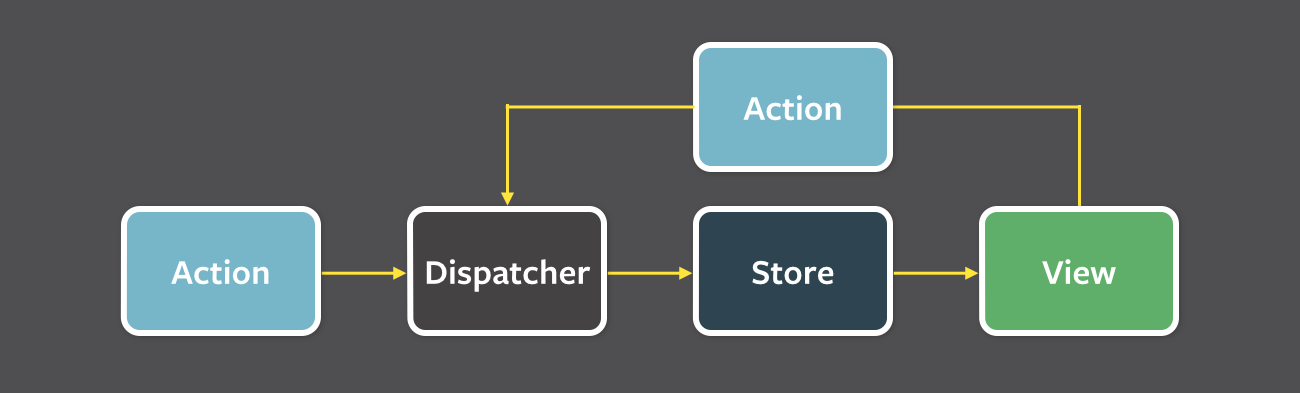
\includegraphics[width=0.9\textwidth]{flux.png}
 \bicaption[fig:longcaptionbad]{Flux 单向数据流}{Flux 单向数据流}{Fig}{Flux Unidirectional Data Flow}
\end{figure}

单向数据流传输的Flux不会像MVC那样,一旦系统复杂了,model和view之间的联系呈几何级数增长,也不会像双向绑定那样,一旦绑定层数多了,连程序员自己都不清楚状态更新是被哪里触发的。

Clarity致力于给用户最好的体验,因此在给合作方做的Smart Home和Smart City两个模块中使用了Flux架构模式。用户也许会在潜意识里感觉到,他们在我们的应用上看到的状态永远是一致的,不会出现类似明明看到有未读的消息点进去却发现没有的情况。

\section{技术架构}
\subsection{前端: Angular VS React}
\subsection{后端: Express VS Koa}
\subsection{数据库: MongoDB和Mongoose}
\subsection{服务器: AWS云服务}

\section{开发工具}
\subsection{IDE: Webstorm VS Atom}
\subsection{版本控制: Git和Git Flow}
\subsection{代码生成: Yeoman和Yeoman Generators}
\subsection{文档生成: JsDoc VS EsDoc}
\subsection{代码质量: Lint工具和Git hooks}
\subsubsection{Eslint}
\subsubsection{Jslint}
\subsubsection{Jscs}
\subsubsection{Stylelint}
\subsubsection{Pre-commit}
\subsection{编译工具: Grunt VS Gulp VS Npm}
\subsection{单元测试: Mocha和Karma}
\subsection{持续集成: Travis-CI VS Solano}



%# -*- coding: utf-8-unix -*-
%%==================================================
%% chapter03.tex
%%==================================================

%\bibliographystyle{sjtu2}%[此处用于每章都生产参考文献]
\chapter{可行性分析}
\label{chap:feasibility}

\section{技术可行性}
\section{资源可行性}

%# -*- coding: utf-8-unix -*-
%%==================================================
%% chapter03.tex
%%==================================================

%\bibliographystyle{sjtu2}%[此处用于每章都生产参考文献]
\chapter{需求分析}
\label{chap:requirement}
本系统分为3个共享数据库的互相关联又相对独立的模块,需求分析的工作不是仅仅做三遍就行,而是要考虑到相互联系和共用资源。由于整体上是传感器管理系统,所以传感器(Sensor)这个资源肯定是共享的,不同的系统都得有登录和权限管理,所以用户(User)也需要共享,这两种资源需要统一在版本管理系统中管理,这样能够保证所有用户和设备资源的一致性,又能在此基础上各自独立地实现业务逻辑。不同系统上的用户可能实际含义不太相同,本系统使用用户的角色(role)属性来区分,具体角色有:
\begin{description}
  \item[普通用户(user)] Smart Home模块和Smart City模块的最终用户,一个传感器会属于一个普通用户,一个普通用户可以拥有多个传感器。
  \item[管理员(admin)] 版本管理模块的最终用户,也就是Clarity的硬件开发人员和管理人员,除了管理传感器版本等信息外还可以管理用户。
  \item[根用户(root)] 超级用户,给系统维护人员或开发人员的角色,拥有最高权限,可以修改任何资源。
\end{description}

注1:本系统中版本管理模块取名“balanar”,Smart Home取名“robotic”,Smart City名字叫“azwraith”。这3个名字都只做内部代号,但也许会在一些代码或截图中出现,为免误解,特此声明。其中只有robotic(意为机器人的)跟项目内容有点联系,其余两个无实际含义。

注2:本章节中的原型和设计稿都不一定与最终的需求吻合,因为可能有些需求修改没有必要在原型和设计稿上体现。

下面本章将详细从不同的角度对各模块进行需求分析:
\section{版本管理模块}
版本管理模块面向的用户是Clarity的硬件开发人员,原本用户使用Excel记录传感器版本、批次、拥有者等信息。但随着传感器的不断改进和零件的不断进货,有越来越多的版本、批次、兼容性、合作方和制作给合作方的特殊版本,使用Excel的时间成本和精力成本越来越高。版本管理模块的最终用户有三种,都是本系统的管理员,分别是软件开发人员、硬件开发人员和公司管理人员。系统需要能够让用户能够处理传感器、用户、兼容性、硬件版本、固件版本、软件版本、五种零件版本和五种零件批次的增删改查以及这些资源之间的复杂关系,还需要处理一些特殊的格式校验,让用户输入的时候得到及时的校验和反馈。

\subsection{用户用例}
本课题使用Power Designer绘制了一个用例图,如图\ref{fig:balanar_usecase}所示,版本管理模块有如下用户用例:
\begin{enumerate}
  \item 所有用户登录;
  \item 硬件开发者增删改查传感器、硬件版本、固件版本、零件版本、零件批次;
  \item 软件开发者增删改查软件版本;
  \item 硬件和软件开发者增删改查版本兼容性;
  \item 公司管理人员增删改查用户;
\end{enumerate}
\begin{figure}[!htp]
 \centering
 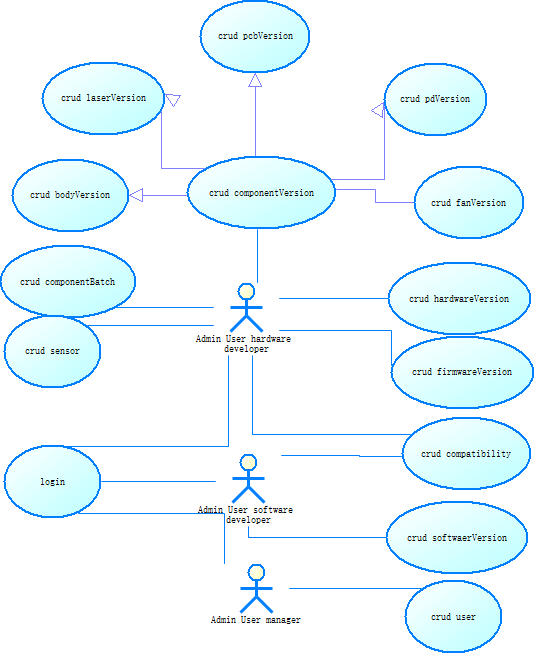
\includegraphics[width=0.8\textwidth]{balanar_usecase.png}
 \bicaption[fig:balanar_usecase]{版本管理模块用例}{版本管理模块用例}{Fig}{Usecase of Version Management}
\end{figure}
\subsection{用户故事}
经过与需求方的多次需求会议,本课题总结出如下主要的用户故事:
\begin{enumerate}
  \item 每当硬件开发人员设计出新版本的零件,需要到系统中添加一个零件版本,填写一些参数,其中ID参数需要严格的格式校验。
  \item 每当硬件开发人员下单订购或者收到一批零件,需要到系统中添加一个零件批次或者修改到货日期,选择相应的一种零件版本。
  \item 每当硬件开发人员准备装配一种拥有新版本零件的传感器,需要到系统中添加一个硬件版本,选择相应的五种零件版本。
  \item 每当硬件开发人员准备装配一种拥有新固件的传感器,需要到系统中添加一个固件版本,并添加对应的兼容性。
  \item 每当硬件开发人员装配完成一批新的传感器,需要到系统中添加这些传感器,选择相应的硬件版本、固件版本和五个零件批次,同时可以指定一个拥有者(普通用户)。
  \item 每当Clarity有新的合作伙伴,Clarity的管理人员可以添加普通用户(角色),将来有给他们专用的传感器时,可以指定为拥有者。
\end{enumerate}
\begin{figure}[H]
 \centering
 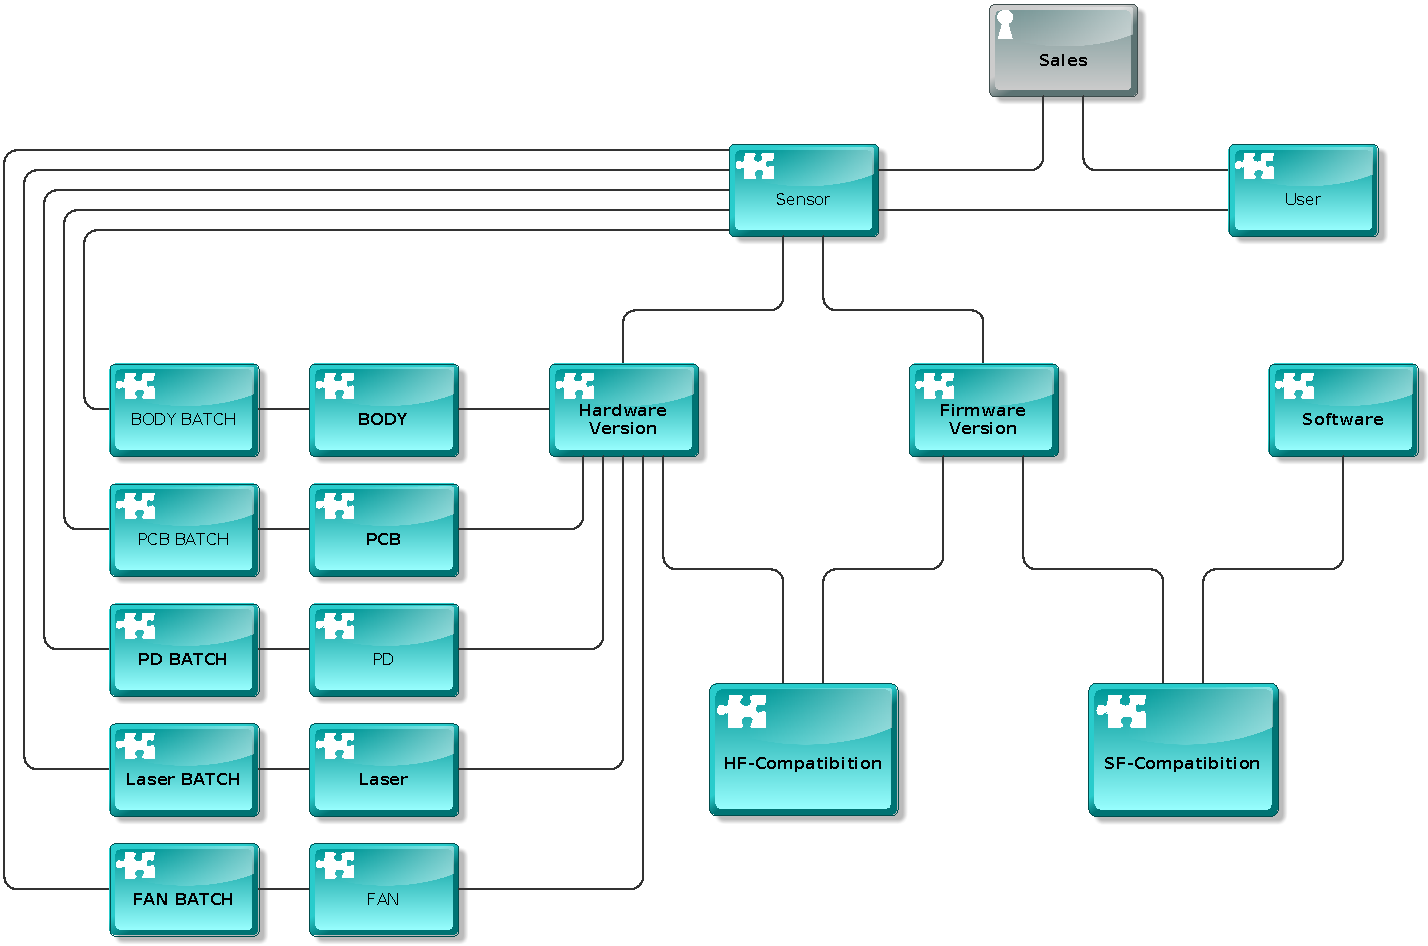
\includegraphics[width=\textwidth]{data_model.png}
 \bicaption[fig:balanar_data_model]{版本管理模块 数据模型}{版本管理模块 数据模型}{Fig}{Version Management module's data model}
\end{figure}
\subsection{数据模型}
本课题使用ARIS业务流程建模软件建立了一个数据模型,如图\ref{fig:balanar_data_model}所示,传感器与硬件版本和固件版本有关,同时与五种零件的批次有光,硬件版本由五种零件版本组成,每个零件版本对于很多零件批次,固件版本和硬件版本有兼容性,固件版本和软件版本有兼容性,每个传感器可以属于一个用户,其中灰色的Sales是不在本模块也不在本系统中的:
\subsection{数据库设计:数据字典}
由于本课题使用的MongoDB不是传统的关系型数据库,数据库表设计不是很有必要,所以直接使用普通文本定义了一套数据字典,以免开发过程中混淆不同的资源名和属性名,同时对字段类型做了一些限定,这里只展示了关于传感器资源的定义,详情请看附录A(数据字典)。
\begin{lstlisting}[language={JSON}, caption={版本管理模块的数据字典}]
Sensor: {
  @pk id
  @fk hardwareVersion
  @fk firmwareVersion,
  @fk componentBatches: {body, pcb, photodiode, laser, fan},

  threshold: type(integer),
  noiseLevel,
  calibrations: {
    mass: type(decimal),
    number: type(decimal)
  },
  applicationType: type(enum(SMART_CITY)),
}
\end{lstlisting}

\subsection{快速原型}
本系统在正式开发之前还使用一款叫做balsamiq模拟软件做了一个快速原型,用于和需求方确认基本的界面和操作流程。如图\ref{fig:balanar_mockup}所示,这里只展示了一个页面,详情请看附录B(快速原型)。
\begin{figure}[H]
 \centering
 \includegraphics[width=\textwidth,page=8]{pdf/balanar_prototype.pdf}
 \bicaption[fig:balanar_mockup]{版本管理模块原型样例}{版本管理模块原型样例}{Fig}{Example mockup of Version Management}
\end{figure}

\section{Smart Home模块}
本模块的当前的主要目标客户是一家日本的家电制造企业,最终用户是该企业家电产品的用户。该企业生产的产品是空调和空气净化器等家用电器,因此Clarity为其量身打造了智能家居(Smart Home)解决方案。
\subsection{智能家居解决方案}
首先,目标用户是购买了该企业各种家电和空气净化器的个人或家庭,用户还可以随身携带一个Clarity的个人空气质量传感器。普通的空气净化器只能一直开着或者在人的操控下间歇性地净化空气,而搭载空气质量传感器的家电也只能检测空气质量并报告给用户,并不能实际改善空气质量,Clarity在两者之间引入了一个烧录了智能程序的可编程扫地机器人巧妙地弥补了两者的不足。

如图\ref{fig:robotic_progress}泳道流程图所示,此智能家居解决方案按以下流程工作:
\begin{enumerate}
  \item 不同房间的空气质量传感器持续上传数据到服务器,服务器保存数据;
  \item 服务器定时地计算并评估空气质量的好坏;
  \item 一旦有房间空气质量低于一定水平,服务器就会给机器人下达净化指令,机器人会移动到对应的房间并开启其上搭载空气净化器;
  \item 空气质量好转之后,服务器再给机器人下达停止指令,机器人会关掉空气净化器原地待命;
  \item 用户可以切换手动模式和自动模式,手动模式下服务器自动指令无效,用户可以指定机器人去某个传感器所在的房间,自动模式下用户控制无效;
\end{enumerate}

\begin{figure}[!htp]
 \centering
 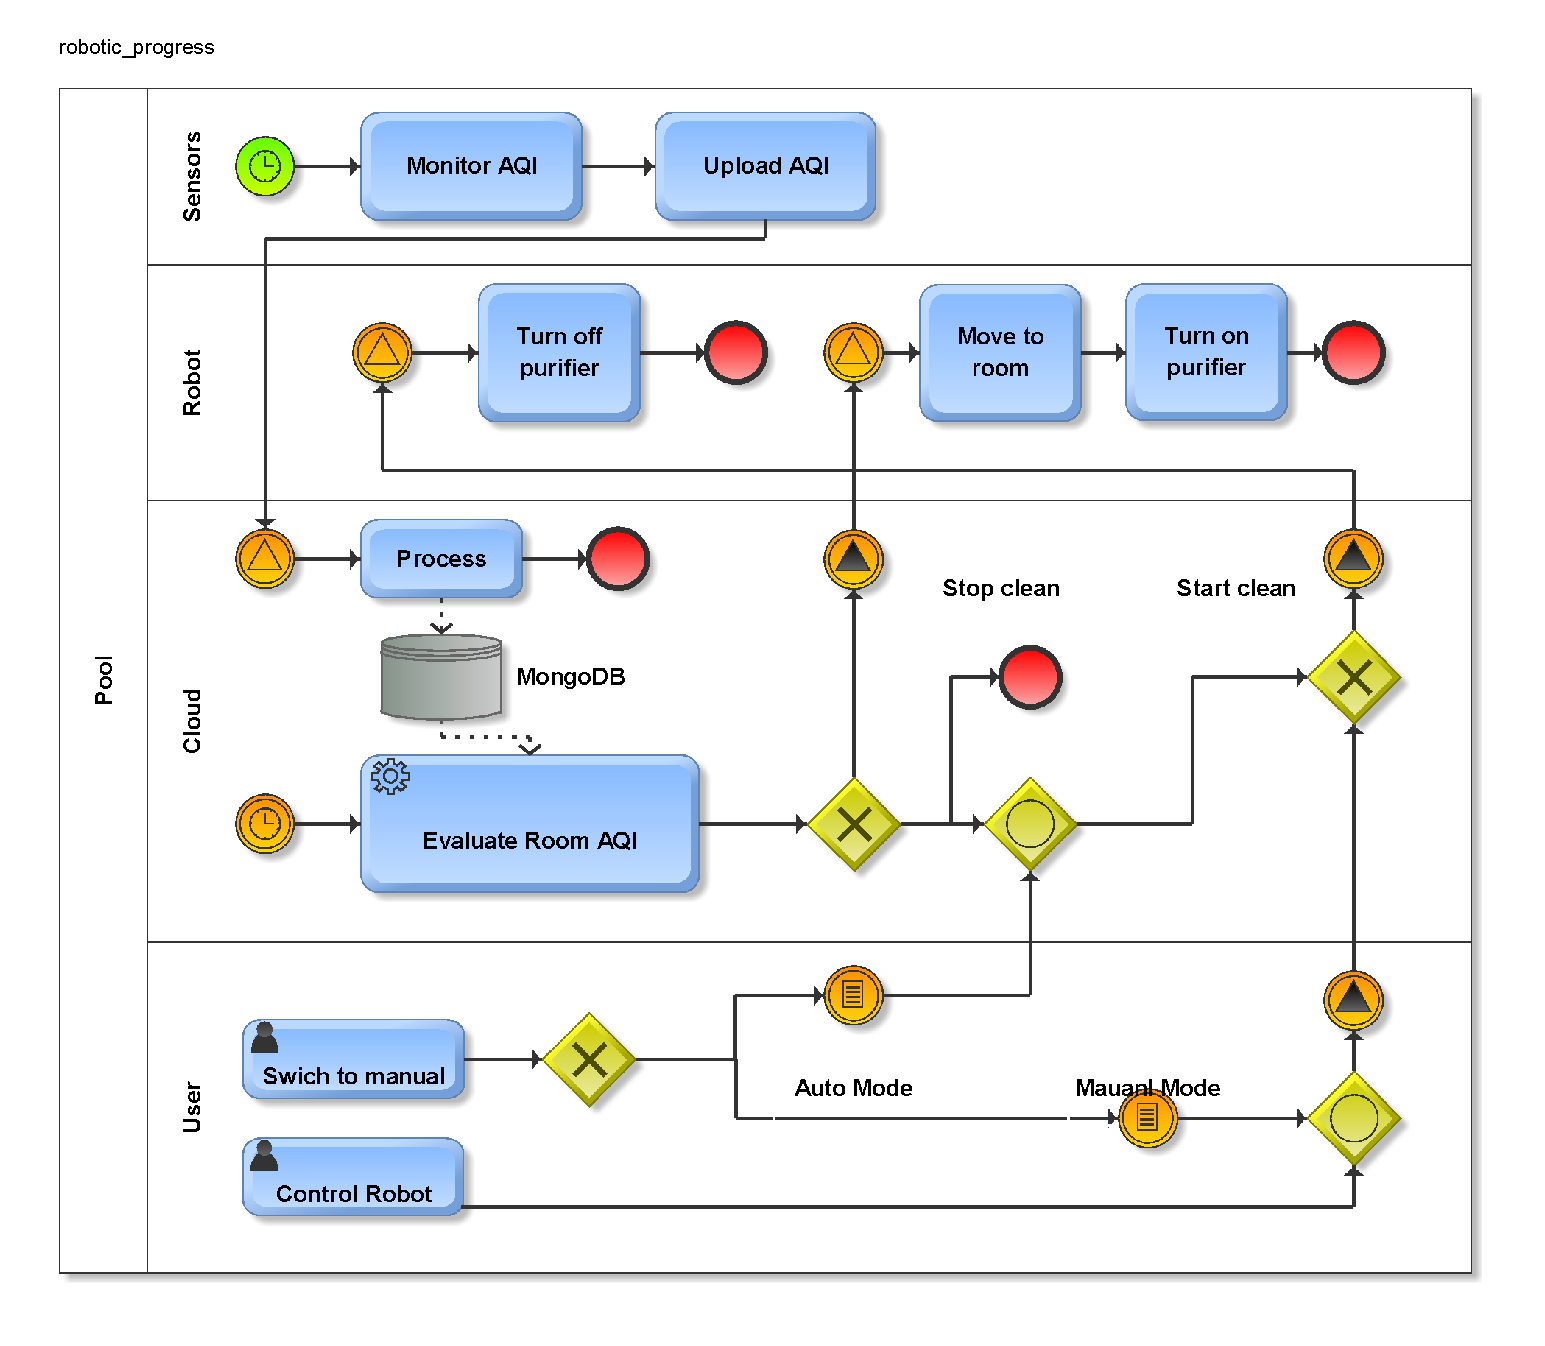
\includegraphics[width=\textwidth]{figure/robotic_progress.pdf}
 \bicaption[fig:robotic_progress]{Smart Home模块泳道流程图}{Smart Home模块泳道流程图}{Fig}{BPMN of Smart Home}
\end{figure}

\subsection{用户用例}
本课题使用Power Designer绘制了一张用例图,如图\ref{fig:robotic_usecase}所示,用户有如下用例:
\begin{itemize}
  \item 登录
  \item 查看空气质量指数(AQI)和健康指数(Health Index)
  \subitem 查看个人AQI和健康指数
  \subitem 查看城市AQI和健康指数
  \subitem 查看家里平均AQI和健康指数
  \subitem 查看家里
  \subsubitem 查看房间空气污染情况
  \subsubitem 查看房间历史AQI折线图
  \item 控制机器人
  \subitem 切换机器人到手动模式或自动模式
  \subitem 控制机器人去某个房间,这一点在界面上依赖查看房间空气质量情况
\end{itemize}
\begin{figure}[!htp]
 \centering
 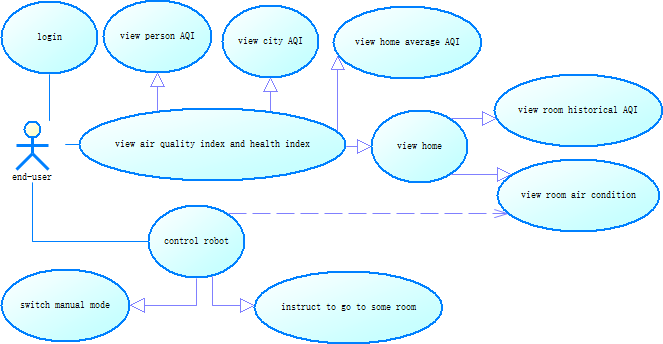
\includegraphics[width=\textwidth]{robotic_usecase.png}
 \bicaption[fig:robotic_usecase]{Smart Home模块用例图}{Smart Home模块用例图}{Fig}{Usecase of Smart Home}
\end{figure}

\subsection{用户故事}
\begin{enumerate}
  \item 用户随时查看个人、家里和城市的空气质量情况和健康指数;
  \item 用户随时家里不同房间的空气质量状况和历史空气质量折线图;
  \item 用户随时查看机器人的位置和空气净化器的工作状态;
  \item 用户随时把机器人切换到手动模式,并控制机器人去任何房间并自动开始净化空气;
\end{enumerate}
\subsection{设计稿}
本模块的需求方给出了一个比较独特且详细的设计稿,如图\ref{fig:robotic_design}所示,这是一个像手风琴一样的页面,个人、家庭、城市三个叶子可以被分别点击展开,这里只展示了一个页面,详情请看附录C(设计稿)。
\begin{figure}[H]
 \centering
 \includegraphics[height=0.8\linewidth, page=2, angle=-90]{pdf/robotic_design.pdf}
 \bicaption[fig:robotic_design]{Smart Home模块设计稿样例}{Smart Home模块设计稿样例}{Fig}{Example design of Smart Home}
\end{figure}

\section{Smart City模块}
本模块的当前主要目标客户是美国一家城市政府,最终用户是政府工作人员。该城市计划大量安装Clarity的传感器以监控城市空气质量,这就需要在智慧城市级别提供空气质量的数据查看和设备管理服务。
\subsection{用户用例}
本课题使用Power Designer绘制了一张用例图,如图\ref{fig:azwraith_usecase},用户具有如下用例:
\begin{enumerate}
  \item 管理设备;
  \subitem 添加设备;
  \subitem 删除设备;
  \subitem 显示设备;
  \subitem 隐藏设备;
  \item 查看数据;
  \subitem 以地图形式查看传感器位置和当前AQI;
  \subitem 以图表形式查看多个设备的最近的AQI,包括实时数据和最新的历史数据;
  \subsubitem 选择时间精度;
  \subsubitem 选择AQI度量;
  \item 保存数据为折线图,此用例依赖以图表形式查看数据的用例;
  \item 导出数据到CSV;
  \subitem 导出最近的AQI数据,此用例依赖以图表形式查看数据的用例;
  \subitem 导出非最近的AQI数据
\end{enumerate}
\begin{figure}[!htp]
 \centering
 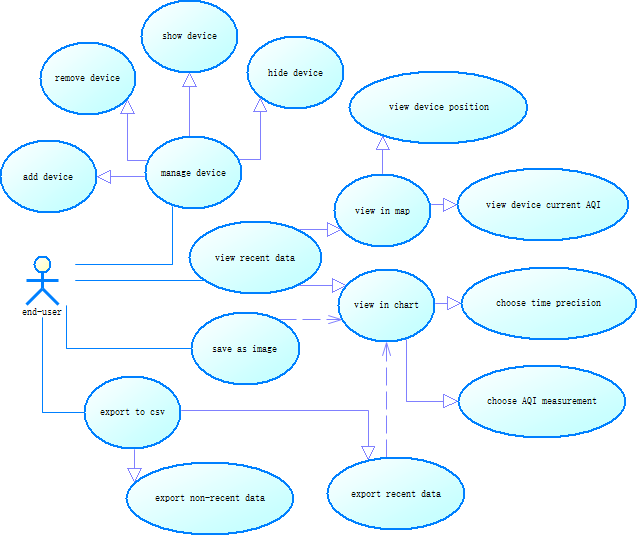
\includegraphics[width=\textwidth]{azwraith_usecase.png}
 \bicaption[fig:azwraith_usecase]{Smart City模块用例图}{Smart City模块用例图}{Fig}{Usecase of Smart City}
\end{figure}

\subsection{用户故事}
\begin{enumerate}
  \item 市政部门安装了新的传感器或者拆除了旧的传感器,用户可以在设备列表中添加或删除设备。
  \item 用户想要查看实时数据或者最近的历史数据,可以在图表中查看,可以在图表中调节时间精度和AQI度量。
  \item 用户想要查看设备的具体位置和当前AQI,可以在地图中查看。
  \item 用户想要在图表或地图中隐藏或显示一些设备,可以在设备列表中勾选或取消勾选。
  \item 用户想要保存当前图表为图片,可以在图表的工具栏中点击保存图片。
  \item 用户想要导出当前图表上的数据,可以在图表的工具栏中点击导出CSV。
  \item 用户想要指定时间段下载,可以在图表的工具栏中点击高级下载跳转到或者直接通过地址进入一个单独的下载页面,在表单中选择设备、时间跨度、时间精度和度量,然后点击下载。
\end{enumerate}

\subsection{快速原型}
本系统在开发之初做了一个简单的快速原型,如图\ref{fig:azwraith_mockups}所示。
\begin{figure}[H]
 \centering
 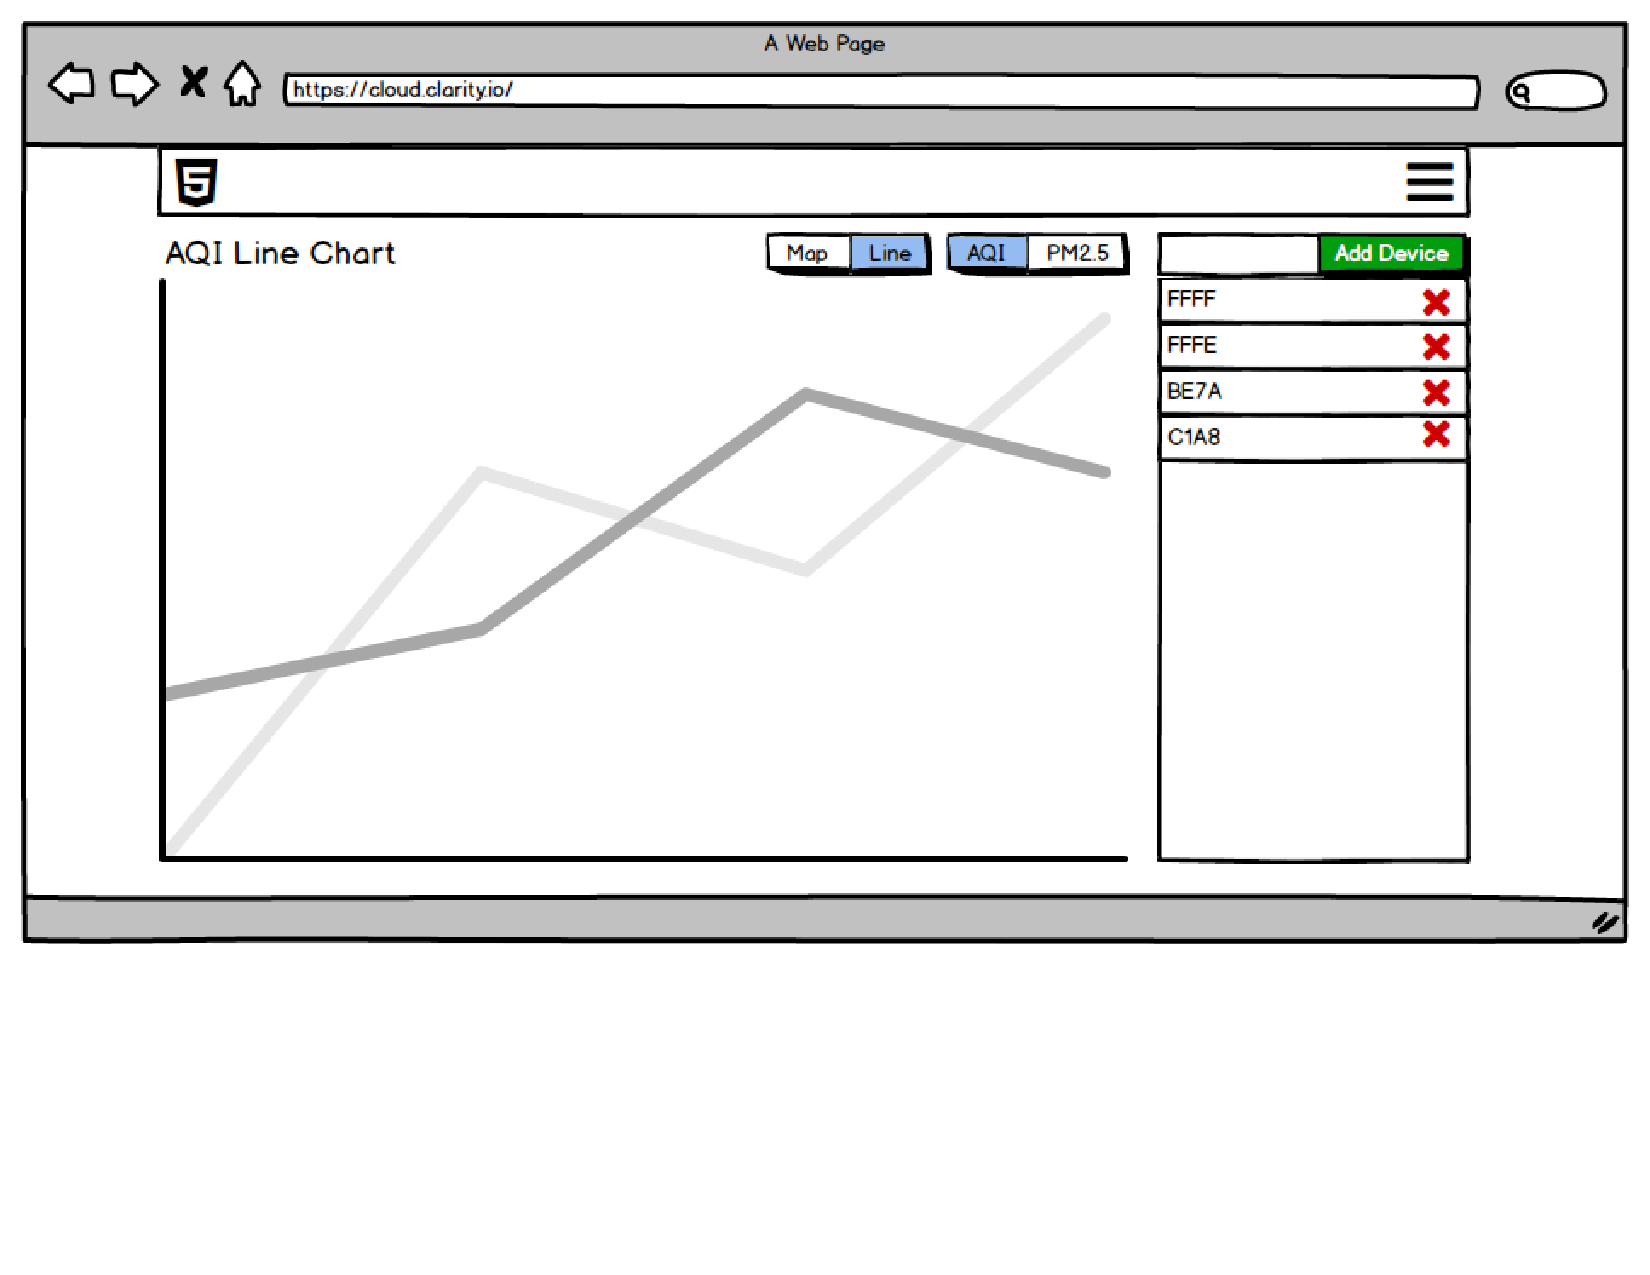
\includegraphics[width=0.7\textwidth]{pdf/azwraith_prototype.pdf}
 
 \vspace{0.1cm}
 
 \includegraphics[width=0.7\textwidth, page=2]{pdf/azwraith_prototype.pdf}
 \bicaption[fig:azwraith_mockups]{Smart City模块原型}{Smart City模块原型}{Fig}{Smart City module’s mockups}
\end{figure}

\subsection{设计稿}
但后来因为这个模块比较重要,而且不像版本管理模块不是非常注重UI,公司又请专门的设计师给出了一个设计稿,如图\ref{fig:azwraith_design}所示。
\begin{figure}[htb]
 \centering
 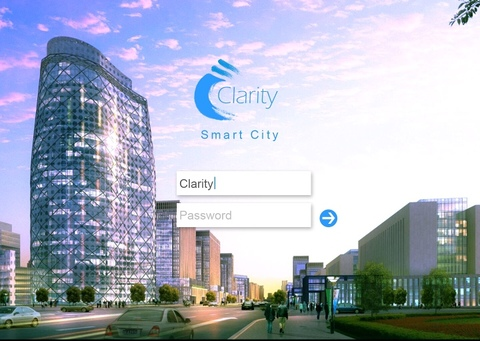
\includegraphics[width=0.75\linewidth]{azwraith_login.jpg}

 \vspace{0.1cm}

 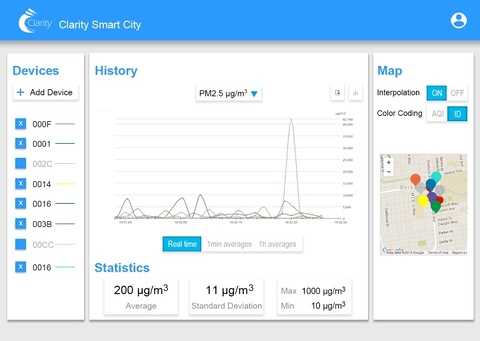
\includegraphics[width=0.75\linewidth]{azwraith_smart_city.jpg}
 \bicaption[fig:azwraith_design]{Smart City模块登录设计稿}{Smart City模块设计稿}{Fig}{Designs of Smart City module}
\end{figure}


%# -*- coding: utf-8-unix -*-
%%==================================================
%% chapter05.tex
%%==================================================

%\bibliographystyle{sjtu2}%[此处用于每章都生产参考文献]
\chapter{系统设计与开发}
\label{chap:design_and_implement}

\section{总体设计}
\subsection{版本管理模块}
\subsection{Smart Home模块}
\subsection{Smart City模块}
\section{版本管理模块}
\subsection{前端}
\subsubsection{客户端ORM}
\subsubsection{代码生成器}
\subsubsection{响应式设计}
\subsection{后端和数据库}
\subsubsection{CRUD Controller}
\subsubsection{on-save实时更新}
\section{Smart Home模块 和 Smart City模块}
\subsection{前端}
\subsubsection{redux管理数据流}
\subsubsection{Echarts绘制图表}
\subsection{后端和数据库}
\subsubsection{socket-io实时更新}
\section{主要组件详细设计}
\subsection{客户端ORM表单组件}
\subsection{EChart组件}
\subsection{AqiChart组件}
\subsection{AqiMap组件}
\subsection{API组件}

%# -*- coding: utf-8-unix -*-
%%==================================================
%% chapter06.tex
%%==================================================

%\bibliographystyle{sjtu2}%[此处用于每章都生产参考文献]
\chapter{系统最终实现效果}
\label{chap:final_effect}

\section{版本管理模块}
\subsection{前端}
\subsubsection{客户端ORM}
\subsubsection{代码生成器}
\subsubsection{响应式设计}
\subsection{后端和数据库}
\subsubsection{on-save实时更新}
\section{Smart Home模块 和 Smart City模块}
\subsection{前端}
\subsubsection{redux管理数据流}
\subsubsection{Echarts绘制图表}
\subsection{后端和数据库}
\section{主要组件详细设计}
\subsection{客户端ORM表单组件}
\subsection{AqiChart组件}
\subsection{AqiMap组件}

%# -*- coding: utf-8-unix -*-
%%==================================================
%% chapter07.tex
%%==================================================

%\bibliographystyle{sjtu2}%[此处用于每章都生产参考文献]
\chapter{系统测试和部署}
\label{chap:test_and_deploy}
本系统对重要的业务逻辑做了单元测试,对整个应用做了端对端测试,然后使用Solano CI做了持续集成,对于生产分支(也就是主分支,master branch),使用了AWS提供的code pipeline服务进行了持续集成。
\section{单元测试}
这里以Smart City模块的redux部分为例,即第\ref{chap:design_and_implement}章中图\ref{fig:redux_dir}所示的Redux文件夹,这一部分是典型的重要业务逻辑。测试主要针对Action Creators和SubReducers函数,在actions.test.js中主要是确保Action Creators会生成正确Action和 Async Action Creators会生成接收dispatch为参数的通用测试,asyncActions.test.js中是对Async Actions Creators的专项测试,各个文件夹中对于每个SubReducers也有对应的测试,确保SubReducers不会修改旧状态(previousState)而且返回正确的新状态(nextState)。

如代码\ref{lst:unit_test}所示,第一个测试检查了所有Action Types变量的值都等于自己的变量名,第二个测试检查了所有Action Types都有一个对于的普通Action Creator会返回这个类型的Action。如图\ref{fig:unit_test}所示,这是Smart City模块的单元测试结果。
\begin{lstlisting}[language={JavaScript}, label={lst:unit_test}, caption={单元测试样例代码}]
describe('redux actionCreators/', () => {
  // ...
  it('each action type\'s value is its name', () => {
    expect(normalActions).to.deep.equal(expectedNormalActionsKeys);
    actionTypes.forEach(actionTypeName => {
      expect(A[actionTypeName]).to.equal(actionTypeName);
    });
  });

  it('each actionType has a corresponding actionCreator returns this type of action', () => {
    expect(actionTypes.length === normalActions.length).to.be.true;
    actionTypes.forEach(actionTypeName => {
      const actionCreatorName = _.camelCase(A[actionTypeName]);
      expect(normalActions).to.include(actionCreatorName);
      expect(A[actionCreatorName]().type).to.equal(actionTypeName);
    });
  });
});
\end{lstlisting}

\begin{figure}[!htp]
 \centering
 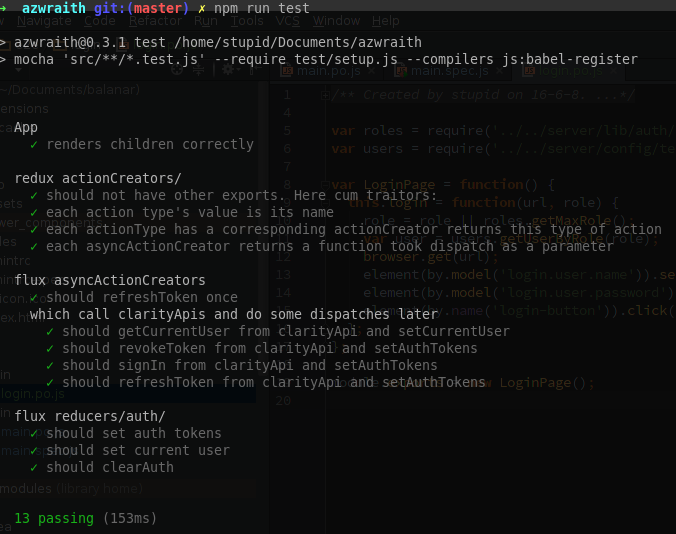
\includegraphics[width=0.8\textwidth]{azwraith_unit.png}
 \bicaption[fig:unit_test]{Smart City模块单元测试结果}{Smart City模块单元测试结果}{Fig}{Unit-test results of Smart City}
\end{figure}
\section{端对端测试}
这里以版本管理模块的端对端测试为例,如代码\ref{lst:e2e_test},如图\ref{fig:e2e_test}

\begin{lstlisting}[language={JavaScript}, label={lst:e2e_test}, caption={端对端测试样例代码}]

\end{lstlisting}

\begin{figure}[!htp]
 \centering
 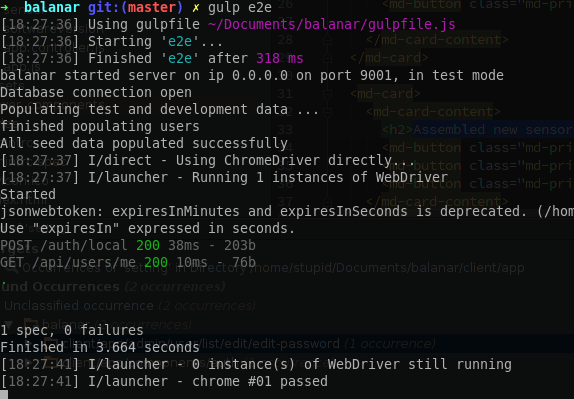
\includegraphics[width=0.8\textwidth]{balanar_e2e.png}
 \bicaption[fig:e2e_test]{版本管理模块端对端测试结果}{版本管理模块端对端测试结果}{Fig}{E2E-test results of Version Management}
\end{figure}

\section{自动部署}
AWS的CodePipeline提供的自动部署一般分为三个步骤,分别是从在线版本管理系统获取新版本的代码,编译代码,然后运行编译结果,在本系统中在线版本管理系统是Github,编译代码部分交给持续集成,最后用Node运行持续集成提交上来的结果。这里以版本管理模块的自动部署为例,如图\ref{fig:code_pipeline}所示这是在AWS上配置了三个步骤的自动部署流程。
\begin{figure}[H]
 \centering
 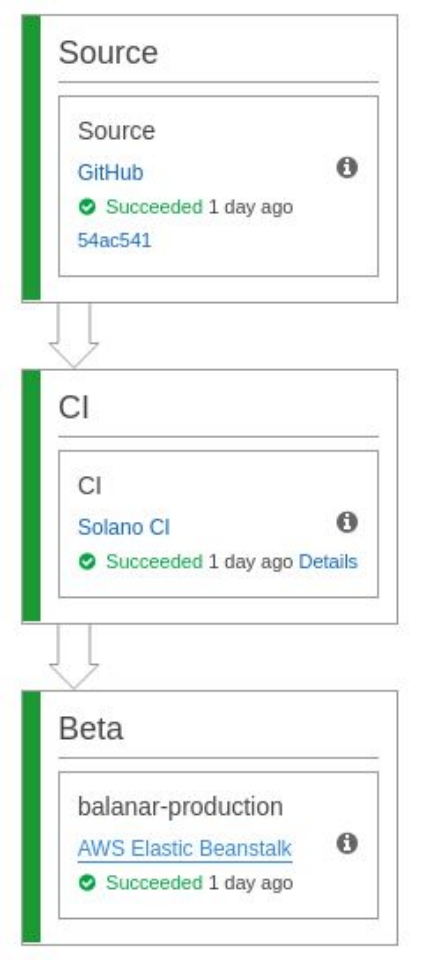
\includegraphics[width=0.4\textwidth]{code_pipeline.jpg}
 \bicaption[fig:code_pipeline]{版本管理模块自动部署流程}{版本管理模块自动部署流程}{Fig}{Code pipeline of Version Management}
\end{figure}

\section{持续集成}
SolanoCI简单的持续集成只需要一个solano.yml配置文件放在项目根目录下面就行了,本系统因为要和AWS的自动部署配合,所以需要在持续集成时进行编译,所以额外使用了一些脚本在solano.yml中调用。这里以Smart City模块的持续集成配置为例,介绍本系统的持续集成情况,该模块因为使用了ES6需要用NodeJS5来编译,而AWS上面只提供了NodeJS4的运行环境,所以持续集成时涉及到多个Node版本的切换,使用了一个叫nvm的库来切换Node版本。如代码\ref{lst:azwraith_ci}所示,持续集成时分2个任务(tests),分别确保进行编译和测试的完成,另有一些钩子(hooks)分布在持续集成的生命周期中:
\begin{description}
  \item[pre-setup] 在启动持续集成之前下载安装nvm并且提前安装好要用的Node4和Node5,最后用Node5安装了执行任务所需要的依赖
  \item[tests] 各个任务会在pre-setup之后post-worker之前执行。
  \item[post-worker] 在每个任务完成后,执行用于发布(--release)的编译(npm run build),并在编译的结果中,使用Node4来安装(npm install)生产环境(--production)的依赖,然后把build文件夹打包并复制到一个特殊的文件夹,SolanoCI之后会把这个文件夹中的内容作为持续集成中这一步的结果上传到服务器上,这样本模块的开发人员就可以下载到持续集成时产生的编译结果,出现错误时方便调试。
  \item[post-build] 在所有任务完成之后,用build文件夹代替了当前文件夹,因为AWS最后会把这个目录作为编译结果。
\end{description}

\begin{lstlisting}[language={JavaScript}, label={lst:azwraith_ci}, caption={Smart City模块持续集成配置}]
hooks:
  pre_setup: bash ./tools/solano/pre-setup.sh
  post_worker: bash ./tools/solano/post-worker.sh
  post_build: bash ./tools/solano/post-build.sh
test_pattern: 'none'
nodejs: false
iojs: false
tests:
  - source ./tools/solano/load-nvm.sh && nvm use 5 && npm run build
  - source ./tools/solano/load-nvm.sh && nvm use 5 && npm test
  
# pre-setup.sh
curl -o- https://raw.githubusercontent.com/creationix/nvm/v0.31.0/install.sh | bash
source ./tools/solano/load-nvm.sh
nvm install 4
npm install -g npm@3
nvm install 5

npm install

# post-worker.sh
source ./tools/solano/load-nvm.sh
nvm use 5

npm run build -- --release

nvm use 4
(cd build && npm install --production)
(cd build && zip -qr ../build.zip .)
cp build.zip $HOME/results/$TDDIUM_SESSION_ID/session/

# post-build.sh
mv build ../
dir=$(pwd -P)
cd ..
rm -rf -- "$dir"
mv build "$dir"
cd "$dir"
\end{lstlisting}

一个SolanoCI的项目会自动监控对应项目的所有分支,不过有自动部署的master分支会由AWS的Code Pipeline来触发持续集成,所以在SolanoCI的配置页面中去掉了master分支。如图\ref{fig:solano}所示,eb开头的持续集成时由AWS的Elastic Beanstalk触发的,dashboard对应的就是azwraith项目的生产环境,普通分支的持续集成时SolanoCI自己触发的。
\begin{figure}[!htp]
 \centering
 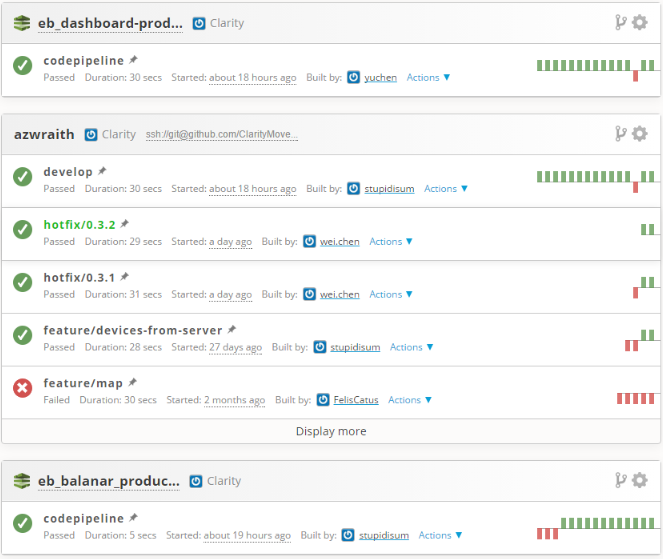
\includegraphics[width=\textwidth]{solano.png}
 \bicaption[fig:solano]{本系统在SolanoCI的持续集成页面}{本系统在SolanoCI的持续集成页面}{Fig}{Dashboard of SolanoCI}
\end{figure}



%# -*- coding: utf-8-unix -*-
%%==================================================
%% chapter08.tex
%%==================================================

%\bibliographystyle{sjtu2}%[此处用于每章都生产参考文献]
\chapter{总结与展望}
\label{chap:summary}

\section{工作总结}

\section{工作展望}



\appendix	% 使用英文字母对附录编号,重新定义附录中的公式、图图表编号样式
\renewcommand\theequation{\Alph{chapter}--\arabic{equation}}	
\renewcommand\thefigure{\Alph{chapter}--\arabic{figure}}
\renewcommand\thetable{\Alph{chapter}--\arabic{table}}
\renewcommand\thealgorithm{\Alph{chapter}--\arabic{algorithm}}

%% 附录内容,本科学位论文可以用翻译的文献替代。

\backmatter	% 文后无编号部分

%% 参考资料
\printbibliography[heading=bibintoc]

%% 致谢、发表论文、申请专利、参与项目、简历
%% 用于盲审的论文需隐去致谢、发表论文、申请专利、参与的项目
\makeatletter

% 致谢页
%# -*- coding: utf-8-unix -*-
\begin{thanks}

  感谢悉心指导论文设计和撰写的指导老师吴刚!

  感谢提携我加入公司并在工作中给出指导和帮助的同事和同学施宇晨!

  感谢在论文写作期间配合延后新需求的CEO陆邓君!

  感谢在工作中通力合作的同事和同学傅浩南!

\end{thanks}
 	  %% 致谢

\makeatother

\end{document}
